% DigitaltechnikFS										Stand: 08.02.2019
% Digitaltechnik Formelsammlung für WiSe 2018/2019			
% 8 Seiten
% Dokumenteinstellungen
% ======================================================================

% Dokumentklasse (Schriftgröße 6, DIN A4, Artikel)
\documentclass[6pt,a4paper]{scrartcl}

% Seitenlayout und Ränder:
\usepackage{geometry}
\geometry{a4paper,landscape, left=6mm,right=6mm, top=0mm, bottom=3mm,includeheadfoot} 

% Dokumentbeschreibung
\title{Digitaltechnik Formelsammlung}
\author{Emanuel Regnath, Martin Zellner, Hendrik Böttcher}

% Pakete laden
\usepackage[utf8x]{inputenc}	% Zeichenkodierung: UTF-8 (für Umlaute)   
\usepackage[german]{babel}		% Deutsche Sprache
\usepackage{multicol}			% Spaltenpaket
\usepackage{amsmath}			% Mathematische Formelzeichen
\usepackage{amssymb}			% Mathematische Formelzeichen
\usepackage{esint}				% erweiterte Integralsymbole
\usepackage{multicol}			% ermöglicht Seitenspalten  
\usepackage{booktabs}			% bessere Tabellenlinien
\usepackage{color}				% Farben
\usepackage{colortbl}			% für die Hintergrundfarbe einzelner Zellen in Tabellen
\usepackage{graphicx}			% Grafiken
\usepackage{pbox}				% Intelligent parbox: \pbox{maximum width}{blabalbalb \\ blabal}
%\usepackage{undertilde}			% Tilde unter Zeichen
\newcommand{\utilde}[1]{#1}
\usepackage{scrtime}			% Uhrzeit
\usepackage{latex4ei_boxes}

%Farben
\definecolor{lightgray}{rgb}{0.8,0.8,0.8}
\definecolor{gray}{rgb}{0.9,0.9,0.9}

% UPDATE WITHOUT CLASS CHANGE
% ----------------------------------------------------------------------

% LastPage
\usepackage{lastpage}

% Allow hyperlinks
	\RequirePackage[pagebackref=true,pdfpagelabels]{hyperref}
	
% Colors
	\RequirePackage{latex4ei/latex4ei_colors}
	\colorlet{col_link}{tum_blue_dark}
	\colorlet{col_sectionbox}{tum_gray}
	\hypersetup{
	colorlinks=true,
	linkcolor=col_link,
	urlcolor=col_link,
	citecolor=col_link,
}

% set pdfoptions
	\AtBeginDocument{
		\hypersetup{
			pdftitle={Digitaltechnik},
	        pdfauthor={Emanuel Regnath, Martin Zellner, Hendrik Böttcher},
	        pdfcreator={LaTeX4EI template (www.latex4ei.de)},
	        pdfkeywords={latex4ei}
	    }
	}

% Date with git commit number
	\newcommand{\themydate}{\today} % Default URL placeholder
	\newcommand{\mydate}[1]{\renewcommand{\themydate}{#1}}	

% Header and Footer
	\RequirePackage{fancyhdr}

	\pagestyle{fancy}
	\fancyhf{}

	\AtBeginDocument{
	\IfFileExists{git.id}{\input{git.id}}{}
	\ifdefined\GitNiceDate\mydate{\GitNiceDate\ (git \GitRevision)}\fi
	\ifdefined\GitIssuesURL
		\ifdefined\setissueslinkurl
		\setissueslinkurl{\GitIssuesURL} % Set the actual URL
		\fi
	\fi
	}
	
% Define Email
	\providecommand{\email}[1]{\href{mailto:#1}{\nolinkurl{#1}}}
	
%
	\renewcommand{\headrulewidth}{0.0pt} %obere Linie ausblenden
	\renewcommand{\footrulewidth}{0.1pt} %obere Linie ausblenden
	
	\newcommand{\issueslinkurl}{https://github.com/latex4ei/Allgemein/issues} % Default URL placeholder
	\newcommand{\setissueslinkurl}[1]{\renewcommand{\issueslinkurl}{#1}}
% ----------------------------------------------------------------------
	
% Schriftart SANS für bessere Lesbarkeit bei kleiner Schrift
\renewcommand{\familydefault}{\sfdefault} 
\renewcommand{\emph}[1]{\textsf{\textbf{#1}}}

% Array- und Tabellenabstände vergrößern
\renewcommand{\arraystretch}{1.2}
\renewcommand{\vec}[1]{\ensuremath{\underline{\boldsymbol {#1}}}}


% Eigene Befehle
\newcommand{\todayV}{\the\day.\the\month.\the\year}                     	    	% Datum D.M.YYYY
\newcommand{\iset}[2]{\ensuremath{\bigl\{ \bigl. #1 \, \bigr| \, #2 \bigr\}}}		% intensional set
\newcommand{\eset}[1]{\ensuremath{\bigl\{#1\bigr\}}}								% extensional set
\newcommand{\norm}[1]{\ensuremath{\|#1\|}}											% Norm
\newcommand{\gk}[1]{\ensuremath{\left\lfloor#1\right\rfloor}} 						% Gaußklammer
\newcommand{\sprod}[2]{\ensuremath{\left\langle #1, #2 \right\rangle }}				% Skalarprodukt
\newcommand{\abs}[1]{\ensuremath{\left\vert#1\right\vert}} 							% Betrag
\newcommand{\mat}[1]{\ensuremath{\begin{bmatrix} #1 \end{bmatrix}}}					% Matrix
\newcommand{\vect}[1]{\ensuremath{\begin{pmatrix} #1 \end{pmatrix}}}				% Vektor
\newcommand{\mvect}[1]{\ensuremath{\left. \begin{matrix} #1 \end{matrix}  \right]}} % Matrixvektor
\newcommand{\ma}[1]{\ensuremath{\utilde{\bs {#1}}}}
\newcommand{\lighthline}{\noalign{\global\arrayrulewidth=0.005pt}\hline\noalign{\global\arrayrulewidth=0.4pt}}

% Abkürzungen
\newcommand{\ul}[1]{\ensuremath{\underline{#1}}}								%Untersteichen
\newcommand{\ol}[1]{\ensuremath{\overline{#1}}}									%Überstreichen
\newcommand{\Ra}[0]{\ensuremath{\Rightarrow}}									%Rightarrow
\newcommand{\ra}[0]{\ensuremath{\rightarrow}} 									%Rightarrow
\newcommand{\n}[0]{\ensuremath{\overline}}										%NOT
\newcommand{\bs}[1]{\ensuremath{\boldsymbol{#1}}}								%Fett und kursiv im mathmode
\newcommand{\diff}{\ensuremath{\ \mathrm d}}									%delta
\newcommand{\grad}{\ensuremath{\mathrm{grad}\ }}								%Gradient
\renewcommand{\div}{\ensuremath{\mathrm{div}\ }}								%Divergenz
\newcommand{\rot}{\ensuremath{\mathrm{rot}\ }}									%Rotation
\newcommand{\Sp}{\ensuremath{\mathrm{Sp}\ }}									%Spur
	% Für Mengen
	\newcommand{\N}{\ensuremath{\mathbb N}}
	\newcommand{\R}{\ensuremath{\mathbb R}}
	\newcommand{\C}{\ensuremath{\mathbb C}}

%Überschreibungen
\renewcommand{\arraystretch}{1.2}
\renewcommand{\vec}[1]{\ensuremath{\underline{\boldsymbol {#1}}}}
\newcommand{\imglog}{\includegraphics[width=.85cm]}


% Dokumentbeginn
% ======================================================================

\begin{document}


% Aufteilung in Spalten
\begin{multicols*}{3}

	% -------------------------------------------
	% | 		Digitaltechik					|
	% ~~~~~~~~~~~~~~~~~~~~~~~~~~~~~~~~~~~~~~~~~~~
	%=======================================================================
	\parbox{2.3cm}{
		
\includegraphics[height=2cm]{img/Logo.pdf}
	}
	\parbox{4cm}{
		\emph{\huge{Digitaltechnik}}
	}

	% ======================================================================
	\section{Boolsche Algebra}

	\subsection{Boolesche Operatoren (Wahrheitstabelle WT)}
	\begin{tabular}{c|c!{\vrule width 1pt}c|c|c|c|c|c}
		  &   & \imglog{img/logic/and-us.png}  & \imglog{img/logic/or-us.png}  & \imglog{img/logic/xor-us.png}  & \imglog{img/logic/nand-us.png}  & \imglog{img/logic/nor-us.png}  & \imglog{img/logic/xnor-us.png}  \\
		  &   & \imglog{img/logic/and-din.png} & \imglog{img/logic/or-din.png} & \imglog{img/logic/xor-din.png} & \imglog{img/logic/nand-din.png} & \imglog{img/logic/nor-din.png} & \imglog{img/logic/xnor-din.png} \\
		  &   & \imglog{img/logic/and-iec.png} & \imglog{img/logic/or-iec.png} & \imglog{img/logic/xor-iec.png} & \imglog{img/logic/nand-iec.png} & \imglog{img/logic/nor-iec.png} & \imglog{img/logic/xnor-iec.png} \\
		x & y & AND                            & OR                            & XOR                            & NAND                            & NOR                            & EQV                             \\
		  &   & $x\cdot y$                     & $x+y$                         & $x\oplus y$                    & $\overline{x\cdot y}$           & $\overline{x+y}$               & $\overline{x\oplus y}$          \\ \hline\hline
		0 & 0 & 0                              & 0                             & 0                              & 1                               & 1                              & 1                               \\ \hline
		0 & 1 & 0                              & 1                             & 1                              & 1                               & 0                              & 0                               \\ \hline
		1 & 0 & 0                              & 1                             & 1                              & 1                               & 0                              & 0                               \\ \hline
		1 & 1 & 1                              & 1                             & 0                              & 0                               & 0                              & 1
	\end{tabular}

	\begin{sectionbox}
		\subsection{Gesetze der booleschen Algebra}
		\begin{tabular}{l|l}
			            & Boolesche Algebra                                                     \\
			            & $({0,1};, +, \overline{a})$                                           \\ \hline
			Kommutativ  & $a b = b a$                                                           \\
			            & $a + b = b + a$                                                       \\ \lighthline
			Assoziativ  & $a (b c) = (a b) c$                                                   \\
			            & $a + (b + c) = (a + b) + c$                                           \\ \lighthline
			Distributiv & $a (b + c) = a b + a c$                                               \\
			            & $a + (b c) = (a + b) (a + c)$                                         \\ \lighthline
			Äquivalenz  & $a a = a$                                                             \\
			            & $a + a = a$                                                           \\ \lighthline
			Absorbtion  & $a (a+b) = a$                                                         \\
			            & $a + (a b) = a$                                                       \\ \lighthline
			Konstanz    & $a 1 = a$                                                             \\
			            & $a + 0 = a$                                                           \\
			            & $a 0 = 0$                                                             \\
			            & $a + 1 = 1$                                                           \\ \lighthline
			Komplement  & $a \overline{a} = 0$                                                  \\
			            & $a + \overline{a} = 1$                                                \\
			            & $\overline{\overline{a}} = a$                                         \\ \lighthline
			De Morgan   & $\overline{a b} = \overline{a} + \overline{b}$                        \\
			            & $\overline{a + b} = \overline{a} \overline{b}$                        \\ \lighthline
			Resolution  & $xa + \overline{x} b$                                                 \\
			(allgemein) & $= x a + \overline{x} b + \textcolor{green}{ab \text{ (Resolvente)}}$ \\
			            & $(x + a) (\overline{x} + b)$                                          \\
			            & $= (x + a) (\overline{x} + b) \textcolor{green}{(a + b)}$             \\ \lighthline
			Resolution  & $xa + \overline{x} a = a$                                             \\
			(speziell)  & $(x + a) (\overline{x} + a) = a$
		\end{tabular}
	\end{sectionbox}


	\subsection{Boolesche Funktionen}
	\begin{equation*}
		f:\{0,1\}^n\ra \{0,1\} \qquad \qquad f(\vec{x})=f(x_1,x_2,\dots,x_n)
	\end{equation*} \\
	Einsmenge $F$ von $f$: $F=\{\vec{x}\in \{0,1\}^n|f(\vec{x})=1\}$ \\
	Nullmenge $\overline F$ von $f$: $\overline F=\{\vec{x}\in \{0,1\}^n|f(\vec{x})=0\}$
	\paragraph{Kofaktor bezüglich}
	\begin{itemize}\itemsep0pt
		\item $x_i: f_{x_i}=f|_{x_i=1}=f(x_1,\dots,1,\dots,x_n)$
		\item $\overline x_i: f_{\overline x_i}=f|_{x_i=0}=f(x_1,\dots,0,\dots,x_n)$
	\end{itemize}
	\paragraph{Substitutionsregel}
	\begin{itemize}\itemsep0pt
		\item $x_i f(\vec{x})=x_i f_{x_{i}}$
		\item $\overline{x}_i f(\vec{x})=\overline{x}_i f_{\overline{x}_{i}}$
		\item $x_i + f(\vec{x})=x_i + f_{\overline{x}_{i}}$
		\item $\overline{x}_i + f(\vec{x})=\overline{x}_i + f_{x_{i}}$
	\end{itemize}
	\paragraph{Boolsche Expansion}
	\begin{itemize}\itemsep0pt
		\item $f(\vec{x})=x_i f_{x_i} + \overline{x}_i f_{\overline{x}_i}$
		\item $f(\vec{x})=(x_i + f_{\overline{x}_i}) (\overline{x}_i + f_{x_i})$
		\item $\overline{f(\vec{x})}=\overline{x}_i \overline{f_{\overline{x}_i}} + x_i \overline{f_{x_i}}$
		\item $\overline{f(\vec{x})}=(\overline{x}_i + \overline{f_{x_i}}) (x_i + \overline{f_{\overline{x}_i}})$
	\end{itemize}
	\paragraph{Eigenschaften von $f(\vec{x})$}
	\begin{itemize}\itemsep0pt
		\item tautologisch $\Leftrightarrow f(\vec{x})=1 \qquad \forall \vec x \in \{0,1\}^n$
		\item kontradiktorisch $\Leftrightarrow f(\vec{x})=0 \qquad \forall \vec x \in \{0,1\}^n$
		\item unabhängig von $x_i \Leftrightarrow f_{x_i} = f_{\overline x_i}$
		\item abhängig von $x_i \Leftrightarrow f_{x_i} \ne f_{\overline x_i}$
	\end{itemize}

	\paragraph{X(N)OR}
	\begin{itemize}
		\item XOR: $a\oplus b=\overline a b + a \overline b$
		\item XNOR: $\overline{a\oplus b} = \overline a \oplus b = a \oplus \overline b =ab + \overline a \overline b = (a+\overline b)(\overline a + b)$
	\end{itemize}

	\subsection{Wichtige Begriffe}
	\begin{tabular}{l|l|l}
		Wichtige Begriffe: & Definition                                                                        & Bemerkung                       \\ \hline
		Signalvariable     & $x$                                                                               & $\hat x \in \eset{0,1}$         \\
		Literal            & $l_i = x_i$ oder $\overline{x_i}$                                                 & $i \in I_0=\eset{1,...,n}$      \\
		Literallänge       & $\#\text{Teilterme}+\sum_{i=1}^{\#\text{Teilterme}}\#\text{Literale v. Teilterm}$ & Summe aller Eingänge            \\
		Minterme,0-Kuben   & M0C $\ni m_j = \prod\limits_{i\in I_0} l_i$                                       & $|$M0C$| = 2^n$                 \\
		d-Kuben            & MC $\ni c_j = \prod\limits_{i\in I_j \subseteq I_0} l_i$                          & $|$MC$|=3^n$                    \\
		Distanz            & $\delta(c_i,c_j) = \bigl| \iset{l}{l \in c_i \land \overline{l}\in c_j}  \bigr|$  & $\delta_{ij} = \delta(c_i,c_j)$ \\
		Implikanten        & $MI = \iset{c \in MC}{c \subseteq f}$                                             &                                 \\
		Primimplikanten    & $MPI = \iset{p \in MI}{p \not\subset c \ \forall c \in MI}$                       & $MPI \subseteq MI \subseteq MC$ \\
	\end{tabular}\\ \\
	\begin{tabular}{l|l|l}
		DNF  & eine Summe von Produkttermen      & Terme sind ODER-verknüpft          \\
		KNF  & ein Produkt von Summentermen      & Terme sind UND-verknüpft           \\
		KDNF & Summe aller Minterme              & WT: 1-Zeilen sind Minterme         \\
		KKNF & Menge aller Maxterme              & WT: 0-Zeilen negiert sind Maxterme \\
		DMF  & Minimale Summe v. Primimplikanten & durch Überdeckungstabelle          \\
	\end{tabular}
	\\ \\

	\section{Beschreibungsformen}
	\subsection{Disjunktive Normalform/Sum of products (DNF/SOP)}
	\textbf{Eins-Zeilen} als \textbf{Implikanten} (UND) schreiben und alle Implikanten mit \textbf{ODER} verknüpfen: \\
	$Z = \overline A \overline B + \overline C D$

	\subsection{Konjunktive Normalform/Product of sums (KNF/POS)}
	\textbf{Null-Zeilen negiert als Implikat} (ODER)  schreiben und alle Implikaten \textbf{UND} verknüpfen: \\
	$Z = ( \ol A + \ol C) ( \ol A + \ol D) ( \ol B + \ol C) ( \ol B + D)$

	\subsection{Umwandlung in jeweils andere Form}
	\begin{enumerate}
		\item Distributivgesetz anwenden (ausmultiplizieren)
		\item Überflüssige Terme streichen (Komplementärgesetz)
		\item Resolventen suchen mithilfe des allg. Resolutionsgesetzes und diese streichen
		\item Mithilfe spez. Resolutionsgesetzes fehlende Terme hinzufügen, bis KKNF/KDNF
	\end{enumerate}
	Oder: Mithilfe Wahrheitstabelle. Hat man z.B. nur 2 Minterme gegeben, so müssen alle anderen Einträge in der Wahrheitstabelle 0 sein und somit Maxterme sein.

	\section{Logikminimierung}
	\subsection{Nomenklatur}
	\begin{itemize}\itemsep0pt
		\item $m_i$ Minterm: UND-Term in dem alle Variablen vorkommen (aus KDNF)
		\item $M_i$ Maxterm: ODER-Term in dem alle Variablen vorkommen (aus KKNF)
		\item $c_i$ Implikant: UND-Term in dem freie Variablen vorkommen können
		\item $C_i$ Implikat: ODER-Term in dem freie Variablen vorkommen können
		\item $p_i$ Primimplikant: UND-Term mit maximal freien Variablen
		\item $P_i$ Primimplikat: ODER-Term mit maximal freien Variablen
		\item $K_{pi}$ Kernprimimplikant: Überdeckt einen Minterm als \textbf{einziger} $c_i$
		\item $K_{Pi}$ Kernprimimplikat: Überdeckt einen Maxterm als \textbf{einziger} $C_i$
	\end{itemize}

	\subsection{Karnaugh-Diagramm} % (fold)
	\textbf{Vorteile}: sehr anschaulich\\
	\textbf{Nachteile}: Gray-Kodierung notwendig, nur wenige Inputvariablen\\
	Zyklische Gray-Codierung: 2dim:$00,01,11,10$ 3dim:$000,001,011,010,110,111,101,100$

	\begin{tabular}{l | c | c |  c | r}
		$_z\!\!\diagdown \!\!^{xy}$ & 00                 & 01                      & 11                      & 10 \\ \midrule
		0                           & 1 \cellcolor{gray} & 0                       & 0                       & 0  \\
		1                           & X \cellcolor{gray} & 1 \cellcolor{lightgray} & 1 \cellcolor{lightgray} & 0  \\
	\end{tabular}
	\begin{minipage}{\linewidth}
		Gleiche Zellen zusammenfassen: z.B. $\overline x \overline y + yz$ \\
		Don't Care Werte ausnutzen!
	\end{minipage}

	% subsection Karnaugh- Diagramm (end)

	\subsection{Quine Methode}
	\textbf{Vorteile}: automatisierbar (DEA/FSM), beliebig viele Inputvariablen\\
	\textbf{Nachteile}: viele paarweise Vergleiche, Erweiterung auf KKNF oder KDNF notwendig, viele Min- und Maxterme\\
	geg.: DNF/KNF oder Wertetabelle von $f(x)$ \\
	ges.: alle Primimplikanten/-kate $p_i$ (VollSOP/VollPOS)  \\ \\
	Spezielles Resolutionsgesetz: $x a + \overline x a = a$ \\
	Absorptionsgesetz: $a + a b = a$

	\begin{enumerate}
		\item kanonische Form (KKNF/KDNF) bestimmen (z.B. $f(x,y,z) = xy = xyz + xy\overline z$)
		\item Alle Min-/Maxterme in Tabelle eintragen (Index von m ist (binär)Wert des Min-/Maxterms), sortieren nach der Anzahl der positiven Literale (=Klasse)
		\item 1-Kubus: Min-/Maxterme die sich um eine Negation unterscheiden, zu einem Term verschmelzen (Resolutionsgesetz), dabei notieren aus welchen 0-Kuben er besteht und alle verwendeten 0-Kuben abhaken
		\item Der 1-Kubus muss zusammenhängend sein! (d.h. alle 1-Kubus Min-/Maxterme müssen zusammenhängen)
		\item Wenn möglich 2-Kubus bilden.
		\item Wenn keine Kubenbildung mehr möglich $\ra$ Nicht abgehakte Kuben sind Primimplikanten
	\end{enumerate}

	\subsection{Überlagerung (Bestimmung der Minimalform)}
	\subsubsection{Mit Mc-Kluskey Überdeckungstabelle bestimmen} Bsp:\\
	\begin{tabular}{|c|c|c|c|c|c|}
		\hline
		          & \multicolumn{4}{c|}{Minterme} &                                      \\ \hline
		Primterme & $m_1$                         & $m_2$   & \dots & $m_N$   & $L(p_i)$ \\ \bottomrule[1pt]
		$p_1$     & $\surd$                       &         &       &         & $L(p_1)$ \\ \hline
		$p_2$     & $\surd$                       &         &       & $\surd$ & $L(p_2)$ \\ \hline
		\vdots    &                               &         &       &         & \vdots   \\ \hline
		$p_K$     &                               & $\surd$ &       &         & $L(p_K)$ \\ \hline
	\end{tabular} \\
	$K$: Anzahl der Primterme\\
	$N$: Anzahl der Minterme \\
	$L(p_i)$: Kosten/Länge der Primimplikanten \vspace{0.1cm}
	\begin{sectionbox}
		\textbf{Vorgehen}:
		\begin{enumerate}
			\item Kernprimimplikanten auswählen (nur ein Kreuz in der Spalte). Zeilen mit Kernprimimplikanten dürfen nicht gestrichen werden!
			\item Spaltendominanzen prüfen und dominierende Spalten streichen (immer Spalte mit mehr Kreuze)\\
			      \begin{tabular}{|c|c|c|c|}
				      \hline
				                & \multicolumn{2}{c|}{Minterme} &         \\ \hline
				      Primterme & $m_1$                         & $m_2$   \\ \bottomrule[1pt]
				      $p_1$     & $\surd$                       & $\surd$ \\ \hline
				      $p_2$     & $\surd$                       & $\surd$ \\ \hline
				      $p_3$     &                               & $\surd$ \\ \hline
				      $p_4$     &                               &         \\ \hline
			      \end{tabular}
			      $m_2$ dominiert $m_1$
			\item Zeilendominanzen prüfen und dominierte Zeilen streichen (immer Zeile mit weniger Kreuze), falls Kosten der dominierten Zeile kleiner als Kosten der dominierenden Zeile sind.
			\item zurück zu 2. falls keine vollständige Überdeckung
		\end{enumerate}
	\end{sectionbox}

	\subsection{Multiplexer}
	\begin{tabular}{ll}
		$f = xa + \overline x b$                                            & (2 Eingänge $a,b$ und 1 Steuereingang $x$)     \\
		$f = \ol x_1 \ol x_2 a + \ol x_1 x_2 b + x_1  \ol x_2 c + x_1 x_2d$ & (Eingänge: $a,b,c,d$  Steuerung: $x_1$, $x_2$) \\
	\end{tabular}
	\subsubsection{Kosten $K_N$ eines N:1 MUX}
	$K_N=N(\log_2(N)+2)$

	\section{Volladdierer (VA)/Ripple-C(u)arry-Adder}
	\parbox{5.0cm}{ 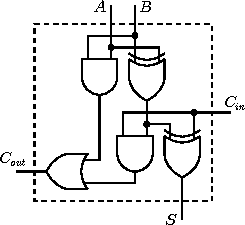
\includegraphics{img/ds/volladdierer.pdf} }
	\hspace*{-.7cm}\parbox{5.0cm}{ 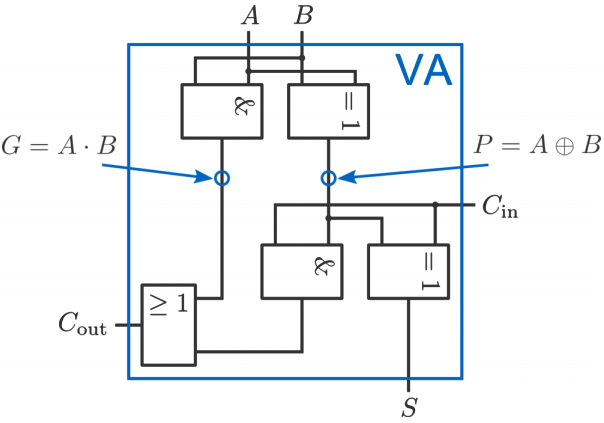
\includegraphics[width=5.0cm]{img/ds/volladdierer-iec.png} } \\
	\textbf{Generate} $g_n = a_n b_n$\\
	\textbf{Propagate} $p_n = a_n \oplus b_n$\\
	\textbf{Summenbit} $S_n = c_n \oplus p_n= a_n \oplus b_n \oplus c_n$\\
	$S_n = \underbrace{a_n\ol{b_n} \ol{c_n} + \ol{a_n}b_n\ol{c_n} + \ol{a_n}\ol{b_n}c_n}_{\text{genau ein Eingang high}} + \underbrace{a_nb_nc_n}_{\text{alle Eingänge high}}$(Ungerade Anzahl von Eingängen 1) \\
	\textbf{Carry-out} $c_{n+1} = c_n p_n + g_n$\\
	$c_{n+1}=\underbrace{a_nb_n\ol{c_n} + a_n\ol{b_n}c_n + \ol{a_n}b_nc_n}_{\text{zwei Eingänge 1}} + \underbrace{a_nb_nc_n}_{\text{drei Eingänge 1}}$ (Mindesten zwei Eingänge 1)
	\\ \\
	\textbf{Laufzeiten (worst case)} \\
	$t_{sn} = \begin{cases} t_{cn} + t_{xor} & t_{cn} > t_{xor} \\ 2 t_{xor} & sonst \end{cases}$\\ \\
	$t_{cn+1} =
		\begin{cases}
			t_{and} + t_{or}           & a_n = b_n = 1 \qquad \qquad (g_n=1)             \\
			t_{xor} + t_{and} + t_{or} & a_n = b_n = 0 \qquad \qquad  (p_n = 0, g_n = 0) \\
			t_{cn} + t_{and} + t_{or}  & a_n \ne b_n \qquad \qquad \qquad  (p_n = 1)
		\end{cases}$\\\\
	Maximaldauer für N-Bit Ripple-Carry-Addierer:\\
	$t_{logic,max}=t_{abc}+(N-2)t_{CC}+\max(t_{cc},t_{cs})$

	\vspace{-3mm}
	\section{Sequentielle Logik}
	\begin{sectionbox}
		\subsection{Begriffe/Bedingungen}
		\begin{tabular}{c|l}
			$t_{Setup}$       & Stabilitätszeit vor der aktiven Taktflanke                                           \\
			$t_{hold}$        & Stabilitätszeit nach  der aktiven Taktflanke                                         \\
			$t_{c2q}$         & Eingang wird spätestens nach $t_{c2q}$ am Ausgang verfügbar                          \\ & ($t_{pd}$ aller Gatter im Register)                           \\
			Min. Taktperiode  & $t_{clk} \ge t_{1,c2q} + t_{logic,max} + t_{2,setup}$                                \\
			Max. Taktfrequenz & $f_{max} = \left\lfloor \frac{1}{t_{clk}} \right\rfloor$ \qquad (Nicht aufrunden)    \\
			Holdzeitbedingung & $t_{2,hold} \le t_{1,c2q} + t_{logic,min}$  $\ra$ Dummy Gatter einbauen              \\
			Durchsatz         & $\frac{\text{Sample}}{t_{clk}}$ \qquad (Sample: Anzahl Eingänge ins letzte Register) \\
			Latenz            & $t_{clk} \cdot (\#$Register $- 1)$ (Anzahl von Logik+Register-Blöcken)               \\ & Zeit, bis Eingangssignal im schlimmsten Fall am letzten Register anliegt.                  \\
		\end{tabular}
	\end{sectionbox}

	\begin{minipage}{\columnwidth}
		\subsection{Pipelining} % (fold)
		Nur bei synchronen(taktgesteuerten) Schaltungen möglich!
		\begin{itemize} \itemsep0pt
			\item Aufteilen langer kombinatorischer Pfade durch Einfügen zusätzlicher Registerstufen\\
			      $\ra$ Möglichst Halbierung des längsten Pfades\\
			      $\ra$ \textbf{neue Registerstufen möglichst so einfügen}, dass $t_{clk,min}=t_{1,c2q}+t_{logic,max}+t_{2,setup}$ halbiert wird (nicht nur $t_{logic,max}$ halbieren!)\\
			      $\ra$ $t_{setup}$ und $t_{c2q}$ des eingefügten Registers beachten. Kann $t_{logic,max}$ auf beiden Seiten des neuen Registers bestimmen.
			\item $t_{hold}$ beachten (evtl. Dummy-Gatter einfügen)
			\item Durchsatz erhöht sich entsprechend der Steigerung der Taktfrequenz
			\item Gesamtlatenz wird eher größer
			\item Taktfrequenz erhöht sich
		\end{itemize}
	\end{minipage}
	% subsection Pipelining (end)

	\subsection{Parallel Processing} % (fold)

	Durchsatz = $\frac{\#\text{Modul}}{t_{clk,Modul}} = f$ \qquad \quad Latenz = $t_{clk}$
	\begin{itemize} \itemsep0pt
		\item Paralleles, gleichzeitiges Verwenden mehrere identischer Schaltnetze
		\item Zusätzliche Kontrolllogik nötig (Multiplexer)
		\item Taktfrequenz und Latenz bleiben konstant
		\item Durchsatz steigt mit der Zahl der Verarbeitungseinheiten \\
		      ABER: deutlich höherer Ressourcenverbrauch
	\end{itemize}
	% subsection Parallel Processing (end)


	\section{Halbleiter}
	\begin{tabular}{l|c|c|c|c|c}
		              & Isolator & Metall    & undotiert   & N-Typ & P-Typ  \\ \hline
		Ladungsträger & Keine    & $e^-$     & $e^- / e^+$ & $e^-$ & $e^+$  \\
		Leitfähigkeit & Keine    & Sehr hoch & $\propto T$ & Hoch  & Mittel \\
	\end{tabular}

	\section{MOS-FET's}
	% ======================================================================
	\textbf{M}etal \textbf{O}xide \textbf{S}emiconductor \textbf{F}ield \textbf{E}ffekt \textbf{T}ransistor\\
	\begin{tabular}{m{4.2cm} m{4.2cm}}
		\begin{minipage}[t]{\linewidth}
			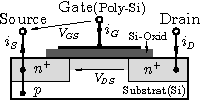
\includegraphics{img/ds/mosfet.pdf} \\[0.2cm]
		\end{minipage} & 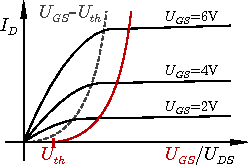
\includegraphics{img/ds/char_nmos.pdf}
	\end{tabular}\\

	\begin{tabular}{l|l}
		\textbf{Bereiche NMOS:}                                                                    \\
		Sperrbereich: $V_{GS} < V_T$                    & Pinch-Off: $V_{DS} = V_{GS} - V_T$       \\
		Lin. Bereich: $0 < V_{DS} < V_{GS} - V_T$       & Sättigung: $V_{DS} > V_{GS} - V_T$       \\ \hline

		\textbf{Bereiche PMOS:}                                                                    \\
		Sperrbereich: $|V_{GS}| < |V_T|$                & Pinch-Off: $|V_{DS}| = |V_{GS}| - |V_T|$ \\
		Lin. Bereich: $0 < |V_{DS}| < |V_{GS}| - |V_T|$ & Sättigung: $|V_{DS}| > |V_{GS}| - |V_T|$ \\
	\end{tabular}

	Kanalabschnürrung (Pinch-Off) immer an der Drain.

	\begin{center}
		\begin{tabular}{c|c}
			\textbf{NMOS Eingangskennlinie}                           & \textbf{PMOS Eingangskennlinie}                           \\
			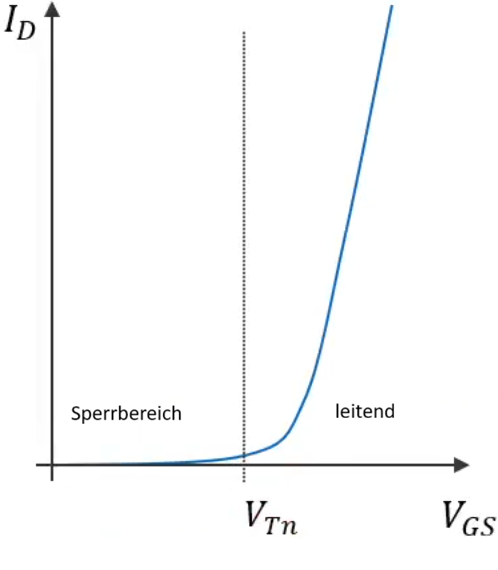
\includegraphics[scale = 0.25]{./img/mos/nmos-input.png}  & 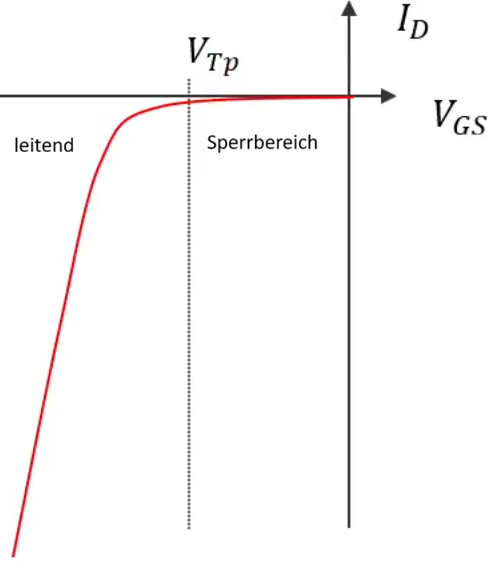
\includegraphics[scale = 0.25]{./img/mos/pmos-input.png}  \\ \hline
			\textbf{NMOS Ausgangskennlinie}                           & \textbf{PMOS Ausgangskennlinie}                           \\
			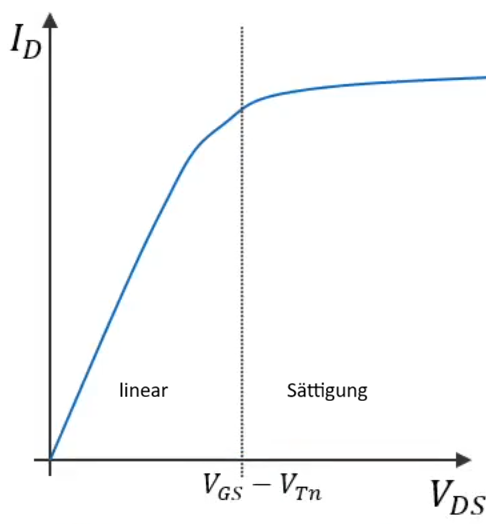
\includegraphics[scale = 0.25]{./img/mos/nmos-output.png} & 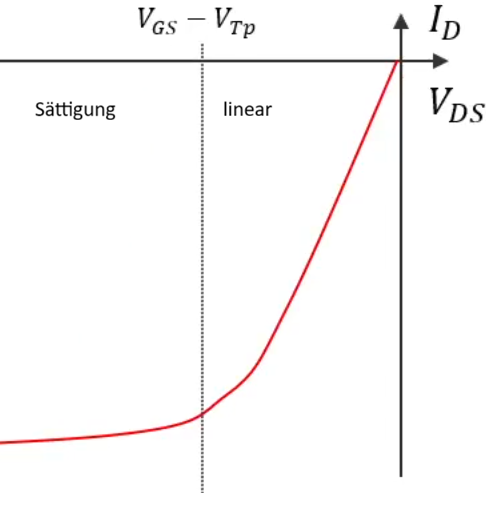
\includegraphics[scale = 0.25]{./img/mos/pmos-output.png}
		\end{tabular}
	\end{center}

	\vspace{-10mm}
	\subsection{Bauteilparameter}
	Verstärkung: \framebox{
		$\beta = K' \frac{W}{L} \text{ mit } K' = \frac{\mu \varepsilon_{ox} \varepsilon_0}{t_{0x}} \qquad [\beta]=\frac{A}{V^2}$
	} \\
	\begin{tabular} {r | l}
		Kanalweite                        & W                                                                                                                        \\
		Kanallänge                        & L                                                                                                                        \\
		Elektronenbeweglichkeit           & $\mu$\quad $\mu_n \approx 250 \cdot 10^{-4} \frac{m^2}{Vs}$, $\mu_p \approx 100 \cdot 10^{-4} \frac{m^2}{Vs}$            \\
		rel. Dielektrizität des Gateoxyds & $\varepsilon_{ox} \approx 3,9$                                                                                           \\
		Dielektrizitätskonstante          & $\varepsilon_0 = 8.8541878 \cdot 10^{-12} \frac{\mathrm{A\,s}}{\mathrm{V\,m}}$                                           \\
		Gateoxyddicke                     & $t_{ox}$                                                                                                                 \\
		Verstärkung                       & $\beta = \frac{\mu_n \varepsilon_{ox} \varepsilon_0}{t_{ox}} \cdot \frac{W}{L} = K' \frac{W}{L} = \frac{\mu_n C_G}{L^2}$ \\
		Kapazität                         & $C_G = \varepsilon_{ox} \varepsilon_0 \frac{WL}{t_{ox}}$                                                                 \\
	\end{tabular}
	\begin{itemize} \itemsep0pt
		\item große Kanalweite $\Ra$ große Drain-Störme \\ $\Ra$ schnelle Schaltgeschwindigkeit (da $i_d \propto \beta \propto \frac{W}{L}$) \\
		      Aber: große Fläche.
	\end{itemize}
	\vspace{-4mm}
	\begin{center}
		\begin{tabular}{cc}
			\textbf{n-Kanal MOSFET} & \raisebox{-.5\height}{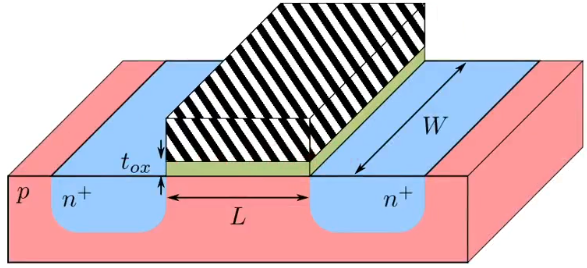
\includegraphics[scale=0.35]{./img/mos/nmos.png}}
		\end{tabular}
	\end{center}
	\begin{minipage}{\columnwidth}
		\subsection{Drainstrom}
		\textbf{nMos} (p-dotiertes Substrat, n-dotierte Drain/Source), schlechter pull up (aufladen der Drain bis $V_{GS} - V_{tn}$) (Pegeldegenerierung)
		\begin{equation*}
			\!\!\! I_d = \begin{cases}
				0,                                                        & V_{GS} < V_{tn} \qquad \qquad  \text{(Sperrber.)}                      \\[0.2em]
				\beta [(V_{GS} - V_{tn}) V_{DS} - \frac{1}{2} V_{DS}^2] , & V_{GS} \ge V_{tn}, 0 < V_{DS} < V_{GS} - V_{tn} \  \text{(lin. Ber.)}  \\\\[0.2em]
				\frac{1}{2} \beta (V_{GS} - V_{tn})^2,                    & V_{GS} \ge V_{tn}, V_{DS} \ge V_{GS} - V_{tn} \  \text{(Sättigungsb.)} \\
			\end{cases}
		\end{equation*}
		\textbf{pMos} (n-dotiertes Substrat, p-dotierte Drain/Source), schlechter pull down (entladen der Drain bis $|V_{tp}|$) (Pegeldegenerierung)
		\begin{equation*}
			\!\!\! I_d = \begin{cases}
				0,                                                          & |V_{GS}| < |V_{tp}|                                       \\[0.2em]
				- \beta [(V_{GS} - V_{tp}) V_{DS} - \frac{1}{2} V_{DS}^2] , & |V_{GS}| \ge |V_{tp}|, 0 < |V_{DS}| < |V_{GS}| - |V_{tp}| \\\\[0.2em]
				- \frac{1}{2} \beta (V_{GS} - V_{tp})^2,                    & |V_{GS}| \ge |V_{tp}|, |V_{DS}| \ge |V_{GS}|-|V_{tp}|     \\
			\end{cases}
		\end{equation*}
	\end{minipage}

	\subsection{pMos und nMos}
	\pbox{3.0cm}{ 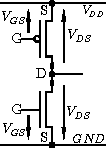
\includegraphics{img/ds/cmos.pdf} }
	\pbox{10.0cm}{
		\begin{tabular}{c|c|c|c}
			Transistor                                    & Source liegt immer am & $V_{GS},V_{DS},I_D$ & Substrat    \\ \midrule
			$\underset{\text{normally on}}{\text{pMos}}$  & höheren Potential     & $\bs{< 0}$          & $+(V_{DD})$ \\
			                                              &                       &                     &             \\
			                                              &                       &                     &             \\
			$\underset{\text{normally off}}{\text{nMos}}$ & niedrigeren Potential & $\bs{> 0}$          & $-(GND)$    \\
		\end{tabular}\\[0.5cm]
	}
	pMos leitet für Gate=GND, nMos leitet für Gate=VDD

	\section{CMOS - Logik}
	% ======================================================================
	\emph{Vorteil:}	 (Fast) nur bei Schaltvorgängen Verlustleistung - wenig statische Verluste \\
	Drei Grundgatter der CMOS-Technologie:\\
	\begin{tabular}{ccc}
		NOT (2 Trans.)                                 & NAND (4 Trans.)                                 & NOR (4 Trans.)                          \\
		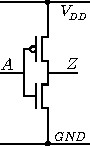
\includegraphics{img/ds/mosfet_not.pdf} \qquad & 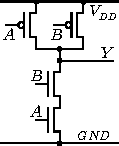
\includegraphics{img/ds/mosfet_nand.pdf} \qquad & 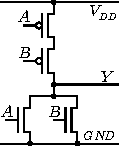
\includegraphics{img/ds/mosfet_nor.pdf} \\
	\end{tabular}\\
	Falls $GND$ und $V_{DD}$ vertauscht würden, dann $NAND \ra AND$ und $NOR \ra OR$\\
	Allerdings schlechte Pegelgenerierung.

	\subsection{Gatterdesign}
	\begin{tabular}{l|l|l}
		Netzwerk      & Pull-Dow\bf{n}    & Pull-U\bf{p}      \\
		Transistoren  & \textbf{n}Mos     & \textbf{p}Mos     \\ \hline
		\textbf{N}AND & Serienschaltung   & Parallelschaltung \\
		\textbf{N}OR  & Parallelschaltung & Serienschaltung   \\
	\end{tabular}\\ \\
	1. Möglichkeit: Direkt; ggf. Inverter vor die Eingänge und Ausgänge schalten.\\
	2. Möglichkeit: Mit boolescher Algebra die Funktion nur mit NAND und NOR darstellen.
	\subsection{CMOS Verlustleistung}
	Inverterschaltvorgang $V_A: 0 \ra 1$:\\
	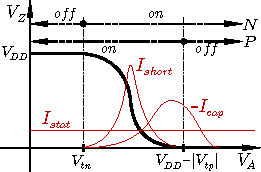
\includegraphics{img/ds/char_inverter.pdf}

	\begin{sectionbox}
		\begin{itemize}
			\item \textbf{Statische Verlustleistung} $I_{stat}$: Minimaler Strom, der zu jeder Zeit durch nMos und pMos fließt (auch im Sperrbereich)
			\item \textbf{Kapazitive Verlustleistung} $I_{cap}$: Verluste, die bei jeder steigenden Flanke des Ausgangs des MOS-Transistors aufgrund der aufzuladenen Kapazitäten auftreten
			\item \textbf{Kurzschlussstrom} $I_{short}$: Strom, der während der kurzen Zeit fließt, wo nMos und pMos beide stark leiten.
		\end{itemize}
	\end{sectionbox}

	\everymath{\displaystyle}
	\emph{Dynamische Verlustleistung} \qquad \ $P_{dyn} = P_{cap} + P_{short}$\\
	\begin{tabular}{ll}
		\quad Kapazitive Verluste \qquad \ \quad \  & $P_{cap} = \alpha_{01} f C_L V_{DD}^2$                                                              \\
		\quad Kurzschlussstrom                      & $P_{short} = \alpha_{01} f \beta_n \tau (V_{DD} - 2V_{tn})^3$                                       \\
		\qquad $\tau$: Zeit, in der beide Transistoren leiten                                                                                             \\[0.8em]
		\quad Schalthäufigkeit                      & $\alpha_{0 \rightarrow 1} = \frac{\text{Schaltvorgänge(pos. Flanke)}}{\text{\# Betrachtete Takte}}$ \\
		\quad Schalthäufigkeit (periodisch)         & $\alpha = \frac{f_\text{switch}}{f_\text{clk}}$                                                     \\
	\end{tabular}\\
	Abhängig von den Signalflanken, mit Schaltfunktionen verknüpft\\
	$\approx \;$ $V_{DD} 1/\propto $ Schaltzeit: $\frac{V_{DD2}}{V_{DD1}} = \frac{t_{D1}}{t_{D2}}$ (bei Schaltnetzen $t_{log}$)\\
	\textbf{Verzögerungszeit} $t_p\propto \frac{C_L}{W(V_{DD}-|V_t|)}$
	\everymath{\textstyle}
	\textbf{Widerstand des MOS im lin. Bereich}\\
	\[
		R_{on,n/p}=\frac{V_{DSn/p}}{I_D}\approx \frac{1}{\beta_{n/p} W(|V_{GSn/p}| - |V_{tn/p}|)}
	\]

	Steigend mit: Kapazitiver Last, Oxiddicke, Kanallänge, Schwellspannung

	Sinkend mit: Kanalweite, Ladungsträger Beweglichkeit, Oxyd Dielektrizität, Versorgungsspannung \\ \\
	\emph{Statische Verlustleistung} $P_{stat}$: Sub-Schwellströme, Leckströme, Gate-Ströme
	Abhängigkeit: $V_{DD}\uparrow:P_{stat}\uparrow$ \qquad $V_{th}\uparrow:P_{stat}\downarrow$ \quad (aber nicht proportional)

	\subsection{CMOS-Dimensionierung}
	$V_{bulk}=V_{\text{p-Kanal}}$ bei nMos und $V_{bulk}=V_{\text{n-Kanal}}$ bei pMos.\\
	Normalerweise ist Potenzial zwischen n-dotiertem und p-dotiertem Bereich gleich GND ($V_{bulk}=0$). Durch Anpassung dieser Spannung kann man unterschiedliche Parameter realisieren:
	\begin{enumerate}
		\item $V_{bulk} < 0 \Rightarrow$ RLZ vergrößert sich \begin{itemize}\itemsep0pt
			      \item $|V_T|$ vergrößert sich
			      \item Verzögerungszeit steigt
			      \item Statische Verlustleistung sinkt
		      \end{itemize}
		\item $0 < V_{bulk} < V_D \Rightarrow$ RLZ verkleinert sich, hebt sich jedoch nicht komplett auf (da $V_{bulk} < V_D$) \begin{itemize}\itemsep0pt
			      \item $|V_T|$ verkleinert sich
			      \item Verzögerungszeit sinkt
			      \item Statische Verlustleistung steigt
		      \end{itemize}
	\end{enumerate}

	\section{Speicherelemente}
	\emph{Flüchtig} Speicherinhalt gehen verloren, wenn Versorgungsspannung $V_{DD}$ wegfällt - Bsp: *RAM\\
	\emph{Nicht Flüchtig} Speicherinhalt bleibt auch ohne $V_{DD}$ erhalten - Bsp: Flash\\
	\emph{Asynchron} Daten werden sofort geschrieben/gelesen.\\
	\emph{Synchron} Daten werden erst mit $clk_{0 \ra 1}$ geschrieben.\\
	\emph{Dynamisch} Ohne Refreshzyklen gehen auch bei angelegter $V_{DD}$ Daten verloren -  Bsp: DRAM\\
	\emph{Statisch} Behält den Zustand bei solange $V_{DD}$ anliegt (keine Refreshzyklen nötig) - Bsp: SRAM\\
	\emph{Bandbreite:} Bitanzahl, die gleichzeitig gelesen/geschrieben werden kann.
	\emph{Latenz:} Zeitverzögerung zwischen Anforderung und Ausgabe von Daten.
	\emph{Zykluszeit:} Minimale Zeitdifferenz zweier Schreib/Lesezugriffe.

	\framebox{$\text{Speicherkapazität} = \text{Wortbreite} \cdot 2^\text{Adressbreite}$ }

	\subsection{Speicherzelle/Register}
	Ring aus zwei Invertern.

	\subsection{Latch (Pegelgesteuert)}
	\parbox{5cm}{
		\emph{Set-Reset Latch:} \\ Zwei gegenseitig rückgekoppelte NAND-Gatter. $0$ an R/S schaltet.
		\\	\emph{Enable-Latch:} ändert Speicherzustand auf $D$ nur wenn $e=1$
	}
	\parbox{.5cm}{\ }
	\parbox{2cm}{
		\begin{tabular}{c|c} e & Q \\ \hline 0 & Q \\ 1 & D \end{tabular}
	}


	\subsection{Flip-Flop (Flankengesteuert)}
	\parbox{5cm}{
		Besteht aus zwei enable-Latches \\
		\emph{Flip-Flop:} Ändert Zustand bei steigender/(fallender) Taktflanke.\\
	}
	\parbox{.5cm}{\ }
	\parbox{2cm}{
		\begin{tabular}{c|c|c} clk & $Q$ & $\ol Q$ \\ \hline $0 \ra 1$ & $D$ & $\ol D$ \\ sonst & $Q$ & $\ol Q$ \end{tabular}
	}

	\section{Block Parity Schaltungen}
	\subsection{Paritätsprüfsumme}
	Konzept zur Absicherung von digitalen Daten durch Anhängen eines Paritätsbits $p$.\\
	- Gerade Anzahl an Einsen im Datenwort: $p = 0$.\\
	- Ungerade Anzahl an Einsen im Datenwort: $p = 1$.\\
	- Realisierung durch XOR-Gatter
	\subsection{Block Parity}
	„Zweidimensionale“ Erweiterung der Paritätsprüfsumme\\
	Beispielblock:\\
	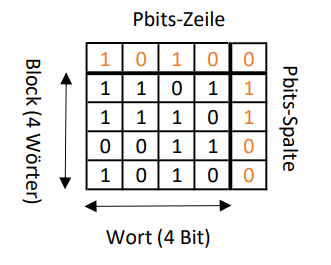
\includegraphics[scale=0.5]{./img/ds/Block_Parity.png}\\
	\textbf{Vorteile:}\\
	- Erkennung und Korrektur von einzelnen Bitfehlern.\\
	- Erkennung von zusammenhängenden Mehrfachfehlern (Bursts).
	\subsection{Realisierung der Block Parity Schaltung}
	\textbf{Datenpfad:}\\ Das n-Bit Datenwort wird durch das Paritybit zu (n+1)-Bit erweitert und übertragen\\
	\textbf{Kontrollpfad:} \\- Die Datenworte (Zeilen im obigen Beispielblock) aus dem Datenpfad werden bitweise verxodert und es entsteht die Pbits-Zeile\\
	- Nach einem Block wird die Pbit-Zeile übertragen



	% subsection Vorgehensweise (end)

	\section{Unwichtiges}
	\begin{itemize} \itemsep0pt
		\item alle 18-24 Monate verdoppelt sich die Anzahl der Transistoren auf gleicher Fläche
		\item Exponentielles Wachstum der Transistorzahl, exponentieller Rückgange des Preises pro Transistor
		\item Herstellungskosten (Fixkosten, Variable Kosten, Technologiefaktor), Entwicklerproduktivität, Verlustleistungsdichte
	\end{itemize}
	\begin{multicols}{3}
		\begin{tabular}{c | c}
			Potenz    & Vorsatz \\ \midrule
			$10^{12}$ & T       \\
			$10^{9}$  & G       \\
			$10^{6}$  & M       \\
			$10^{3}$  & k       \\
			$10^{2}$  & h       \\
			$10^{1}$  & da
		\end{tabular}
		\begin{tabular}{c | c}
			Potenz     & Vorsatz \\ \midrule
			$10^{-1}$  & d       \\
			$10^{-2}$  & c       \\
			$10^{-3}$  & m       \\
			$10^{-6}$  & $\mu$   \\
			$10^{-9}$  & n       \\
			$10^{-12}$ & p       \\
			$10^{-15}$ & f
		\end{tabular}
		\begin{tabular}{ r | l }
			$Hz$      & $s^{-1}$            \\
			N         & $kg m s^{-2} $      \\
			$J $      & $ N m = V A s$      \\
			$W $      & $ V A  = J s^{-1} $ \\
			$ C $     & $ A s $             \\
			$V $      & $ J C^{-1} $        \\
			$F $      & $ C V^{-1} $        \\
			$\Omega $ & $ V A^{-1} $        \\
			$ H $     & $ V s  A^{-1}$
		\end{tabular}
	\end{multicols}
	$Bit \xrightarrow{\cdot 8} Byte \xrightarrow{\cdot 1024} kByte \xrightarrow{\cdot 1024} MByte$

	\section{pn-Übergang}
	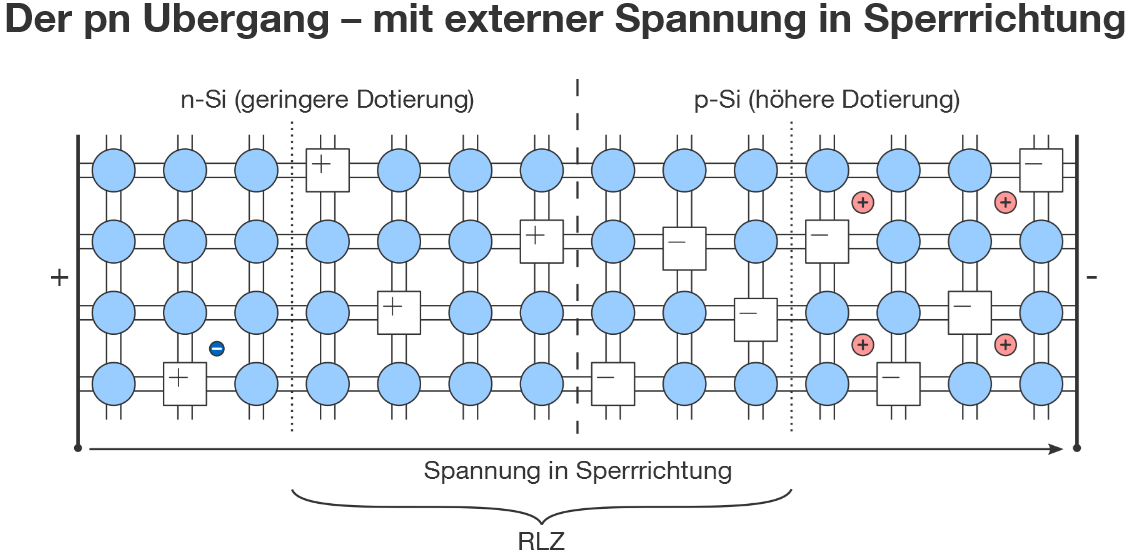
\includegraphics[scale = .4]{./img/mos/pn.png}

	% Ende der Spalten
\end{multicols*}
% Dokumentende
% ======================================================================
\end{document}
